\documentclass[12pt]{article}
\usepackage{amssymb}
\usepackage{geometry}
\usepackage{graphicx}
\usepackage[colorlinks=true, allcolors=blue]{hyperref}
\usepackage{cite}
\usepackage{wrapfig}
\usepackage{booktabs}
\usepackage{soul}
\usepackage[most]{tcolorbox}
\usepackage{amsmath}
\usepackage{lipsum}
\usepackage{caption}
\usepackage{ulem}
\usepackage{xcolor}
\usepackage{tikz}
\usetikzlibrary{arrows.meta, positioning, shapes}
\usepackage{sectsty}

%--------- Define Colors ---------
\definecolor{titleColor}{HTML}{800000}        % Maroon
\definecolor{sectionColor}{HTML}{4682B4}      % SteelBlue
\definecolor{subsectionColor}{HTML}{6A5ACD}   % SlateBlue
\definecolor{textHighlight}{HTML}{DAA520}     % Goldenrod
\definecolor{backgroundColor}{HTML}{F0F8FF}   % AliceBlue
\definecolor{emphasisColor}{RGB}{200, 50, 50} % ForestGreen

\sectionfont{\color{sectionColor}}       % Color for \section
\subsectionfont{\color{subsectionColor}} % Color for \subsection

%--------- Custom Highlight Commands ---------
\definecolor{lightblue}{RGB}{230, 240, 255}
\definecolor{lightgreen}{RGB}{220, 255, 220}
\definecolor{lightred}{RGB}{255, 230, 230}
\definecolor{lightyellow}{RGB}{255, 255, 200}
\definecolor{darkblue}{RGB}{0, 51, 102}

\newcommand{\bluehighlight}[1]{\colorbox{lightblue}{#1}}
\newcommand{\greenhighlight}[1]{\colorbox{lightgreen}{#1}}
\newcommand{\redhighlight}[1]{\colorbox{lightred}{#1}}
\newcommand{\yellowhighlight}[1]{\colorbox{lightyellow}{#1}}
\newcommand{\blue}[1]{\textcolor{darkblue}{#1}}
\newcommand{\myemphasis}[1]{\textcolor{emphasisColor}{\textbf{#1}}}

%--------- Color Blocks ---------
\newtcolorbox{blockA}{
  breakable,
  colback=blue!5,
  colframe=blue!40!black,
  enhanced,
  boxrule=0.7pt,
  arc=2mm,
  left=4mm,right=4mm,top=2mm,bottom=2mm
}

\newtcolorbox{blockB}{
  breakable,
  colback=red!5,
  colframe=red!40!black,
  enhanced,
  boxrule=0.7pt,
  arc=2mm,
  left=4mm,right=4mm,top=2mm,bottom=2mm
}

\newtcolorbox{blockC}{
  breakable,
  colback=green!5,
  colframe=green!40!black,
  enhanced,
  boxrule=0.7pt,
  arc=2mm,
  left=4mm,right=4mm,top=2mm,bottom=2mm
}

\newtcolorbox{blockD}{
  breakable,
  colback=purple!5,
  colframe=purple!40!black,
  enhanced,
  boxrule=0.7pt,
  arc=2mm,
  left=4mm,right=4mm,top=2mm,bottom=2mm
}

%--------- Title ---------
\title{\textcolor{titleColor}{\textbf{\Huge Google Sites Research Portal Layout }}}
\author{B. M. Osman\thanks{Al Nahada University, Cairo \\ \texttt{babikerosman@yahoo.com}}}
\date{\today}

\begin{document}
\maketitle



\begin{center}
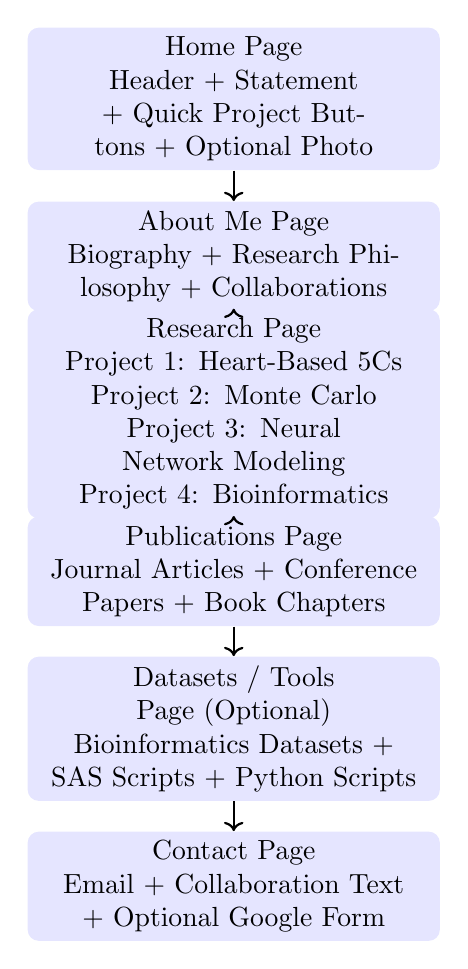
\begin{tikzpicture}[node distance=2cm, every node/.style={fill=blue!10, rounded corners, text width=5cm, align=center}]
% Nodes
\node (home) {Home Page \\ Header + Statement + Quick Project Buttons + Optional Photo};

\node[below of=home] (about) {About Me Page \\ Biography + Research Philosophy + Collaborations};

\node[below of=about] (research) {Research Page \\ Project 1: Heart-Based 5Cs \\ Project 2: Monte Carlo \\ Project 3: Neural Network Modeling \\ Project 4: Bioinformatics};

\node[below of=research] (pub) {Publications Page \\ Journal Articles + Conference Papers + Book Chapters};

\node[below of=pub] (data) {Datasets / Tools Page (Optional) \\ Bioinformatics Datasets + SAS Scripts + Python Scripts};

\node[below of=data] (contact) {Contact Page \\ Email + Collaboration Text + Optional Google Form};

% Arrows
\draw[->, thick] (home) -- (about);
\draw[->, thick] (about) -- (research);
\draw[->, thick] (research) -- (pub);
\draw[->, thick] (pub) -- (data);
\draw[->, thick] (data) -- (contact);

\end{tikzpicture}
\end{center}

\end{document}

